\begin{figure}[!htbp]
\centering
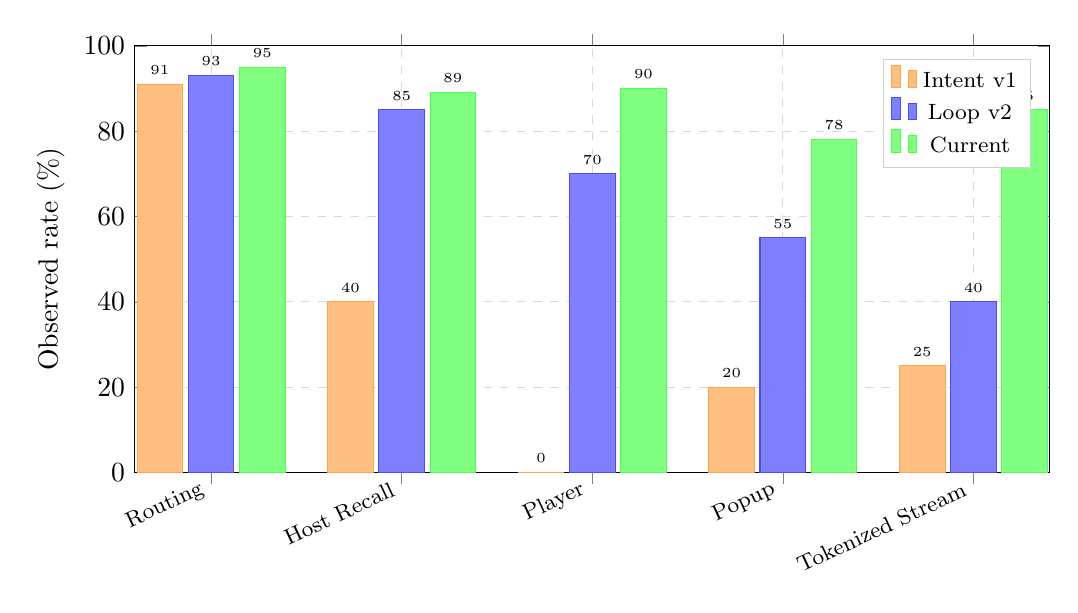
\begin{tikzpicture}
\begin{axis}[
  ybar,
  bar width=0.58cm,
  width=13.2cm, height=7.0cm,
  symbolic x coords={Routing, Host Recall, Player, Popup, Tokenized Stream},
  xtick=data,
  x tick label style={rotate=25, anchor=east, font=\footnotesize},
  ymin=0, ymax=100,
  ylabel={Observed rate (\%)},
  legend style={at={(0.98,0.97)}, anchor=north east, font=\footnotesize, draw=gray!35, fill=white},
  nodes near coords,
  every node near coord/.append style={font=\tiny},
  grid=major, grid style={dashed, gray!30}
]
\addplot[fill=orange!50, draw=orange!70] coordinates {
  (Routing,91)(Host Recall,40)(Player,0)(Popup,20)(Tokenized Stream,25)
};
\addplot[fill=blue!50, draw=blue!70] coordinates {
  (Routing,93)(Host Recall,85)(Player,70)(Popup,55)(Tokenized Stream,40)
};
\addplot[fill=green!50, draw=green!70] coordinates {
  (Routing,95)(Host Recall,89)(Player,90)(Popup,78)(Tokenized Stream,85)
};
\legend{Intent v1, Loop v2, Current}
\end{axis}
\end{tikzpicture}
\caption{Regression-batch improvement across the main browser-agent KPIs.}
\label{fig:manual-kpi-bars}
\end{figure}
